
\chapter{No-Regret Learning}\label{chapter:noRegretLearning}

Regret dynamics are one the best studied algorithmic frameworks in online convex optimization. They not only apply in Game Theory but also in Machine Learning and Information Theory. In this chapter the concept of no-regret Learning will be introduced similar to \cite[Chapter 2]{HDRmertikopoulos}. Later we will cover two concrete no-regret algorithms, namely \textit{projected online gradient descent} and \textit{entropic gradient descent}. In the simulations of chapter \ref{chapter:simulations} we will then run those two algorithms on simple finite games. Note that throughout chapter \ref{chapter:noRegretLearning} we will minimize losses, which is the convention in optimization. In the chapter \ref{chapter:finiteGames}, on the other hand, we are maximizing utilities, which is the convention in game theory.


\section{Notation and Basic Definitions}\label{section:notationAndDefinitionsRegret}

Lets first define some basic concepts that we will make use of. Throughout sets are denoted by upper case letters and vectors by lower case letters. In Online Learning a sequence of play is considered. Therefore, we denote $x_t$ the $t$-th vector in the sequence of $x_1, \dots, x_T$ where $T$ is the number of iterations. \\
The \textit{inner product} of two vectors $x$ and $y$ with dimension $n$ is defined as 

\begin{equation*}
    \langle x,y\rangle = \sum_{i=1}^{n}x_i y_i
\end{equation*}

The \textit{norm} $l_p$ of a vector $x$ is defined as

\begin{equation*}
    \|x\|_p = (\sum_{i}(|x_i|^p)^{1/p}
\end{equation*}

In particular the $l_2$ (or Euclidean) norm is then $\|x\|_2 = \sqrt{\langle x,x\rangle}$. \\

The \textit{gradient} of a differentiable function $f: \mathcal{X} \to \mathbb{R}$ is denoted by $\nabla f$. A function $f$ is called $L-$\textit{Lipschitz} over a set $\mathcal{X}$ with respect to some norm $\|\cdot\|$ if for all $x,y \in \mathcal{X}$ we have that, 

\begin{equation*}
    |f(x) - f(y)| \le L\|x - y\|
\end{equation*}

A function $f:\mathcal{X} \to \mathbb{R}$ is said to be \textit{convex} if for all $x,y$ and $\lambda \in [0,1]$ we have that 

\begin{equation*}
    f(\lambda x + (1-\lambda)y) \le \lambda f(x) + (1-\lambda)f(y)
\end{equation*}

Equivalently, a function $f:\mathcal{X} \to \mathbb{R}$ is said to be \textit{concave} if for all $x,y$ and $\lambda \in [0,1]$ we have that 

\begin{equation*}
    f(\lambda x + (1-\lambda)y) \ge \lambda f(x) + (1-\lambda)f(y)
\end{equation*}

A function $f:\mathcal{X} \to \mathbb{R}$ is $\sigma-$\textit{strongly-convex} over $\mathcal{X}$ with respect to some norm $\|\cdot\|$ if the is some $x \in \mathcal{X}$ such that for all $y \in \mathcal{X}$ we have 

\begin{equation*}
    f(y) \ge f(x) + \langle\nabla f(x),y - x\rangle + \frac{\sigma}{2}\|y - x\|^2
\end{equation*}

A set is called \textit{convex} if for all $x,y \in \mathcal{X}$ and $\lambda \in [0,1]$ we have that 
\begin{equation*}
    \lambda x + (1-\lambda)y \in \mathcal{X} 
\end{equation*}

Throughout this paper $\mathcal{V}$ will denote a finite-dimensional real space with some norm $\|\cdot\|$ and $\mathcal{X} \subset \mathcal{V}$ a closed convex subset thereof. We will write ri($\mathcal{X}$) as the relative interior of $\mathcal{X}$, bd($\mathcal{X}$) for its boundary and diam($\mathcal{X}$) $ = $ sup$\{\|x-x'\|: x,x' \in \mathcal{X}\}$) for its diameter. Also we will denote $\mathcal{Y} \equiv \mathcal{V}^*$ for the algebraic dual of $\mathcal{V}$, $\langle y,x \rangle$ for the canonical pairing of $y \in \mathcal{Y}$ and $x \in \mathcal{V}$ and $\|y\|_* \equiv $ sup$\{\langle y,x \rangle: \|x\| \le 1\}$ for its dual norm. Given an extended real-valued function $f: \mathcal{V} \to \mathbb{R} \cup \{+\infty\}$ its effective domain is defined as dom$f = \{x \in \mathcal{V} : f(x) < \infty\}$.


\section{The Basic Model}\label{section:theBasicModel}

In online optimization the goal is to minimize the aggregate loss incurred against a sequence of unknown loss functions. Formally, at every time step $t = 1, \dots T$ the optimizer selects an \textit{action} $x_t$ from a closed convex subset $\mathcal{X}$ of an $n$-dimensional normed space $\mathcal{V}$. After that the optimizer suffers a loss convex $l_t(x_t)$ based on an a priori unknown loss function $l_t:\mathcal{X} \to \mathbb{R}$. Based on that the optimizer then updates it action and repeats. See figure \ref{fig:OCO} for a pseudo code.\\

\begin{figure}[H]\centering
    \textit{Online Convex Optimization}
    \begin{minipage}{.9\linewidth}
        \begin{algorithm}[H]
        \DontPrintSemicolon
        \KwInput{convex action set $\mathcal{X}$, sequence of convex loss functions $l_t:\mathcal{X} \to \mathbb{R}$ }
        \For{$t = 1,2,\dots,$T} {
        select action $x_t \in \mathcal{X}$ \;
        incur loss $l_t(x_t)$ \;
        update $x_t \gets x_{t+1}$ \;
        }
        \end{algorithm}\caption{pseudo code for the online convex optimization framework}  \label{fig:OCO}
  \end{minipage}
\end{figure}

Based on properties of the loss function we distinguish between two disjoint subclasses of online optimization. Throughout we assume $l_t$ to be differntiable and that it attains a minimum in $\mathcal{X}$.

\begin{enumerate}
    \item\label{item:stronglyOptimization} \textit{Online strongly convex optimization}: each $l_t$ is assumed to be strongly convex, i.e.
    \begin{equation}\label{equ:stronglyOptimization}
        l_t(x') \ge l_t(x) + \langle \nabla l_t(x),x'-x\rangle + \frac{\alpha_t}{2}\|x'-x\|^2
    \end{equation}
    for some $\alpha_t > 0$
    \item \textit{Online linear optimization}: each $l_t$ is assumed to be linear, i.e. 
    \begin{equation}\label{equ:linaerOptimization}
        l_t(x) = -\langle v_t,x\rangle
    \end{equation}
    for some \textit{payoff vector} $v_t \in \mathcal{V}^*$
\end{enumerate}

Depending on the information available to the optimizer we can specify two feedback assumptions:

\begin{enumerate}
    \item \textit{Full information}: the entire loss function $l_t$ is revealed to the optimizer at each time step.
    \item \textit{First order information}: only the perfect gradient $\nabla l_t(x_t)$ for some input $x_t \in \mathcal{X}$ is revealed. 
\end{enumerate}

Obviously \textit{first order information} is a much lighter assumption than \textit{full information} and therefore applicable to a wider range of problems. 


\section{Regret Minimization}\label{section:regretMinimization}

The notion of \textit{regret} is a widely used performance measure of online algorithms. In words, it measures how "sorry" the optimizer is, to not have followed
a fixed competing action in hindsight. It is the difference between the cumulative loss
of the actual sequence of play induced by an algorithm and the cumulative loss of the best fixed action.

\begin{definition}\label{def:regret}
    The \textit{regret} incurred by a sequence of \textit{actions} $x_t \in \mathcal{X}$ and a sequence of loss functions $l_t:\mathcal{X} \to\mathbb{R}$ for an algorithm running for $T$ iterations is defined as
    \[reg(T) = \sum_{t=1}^T l_t(x_t) - \min_{x \in \mathcal{X}} \sum_{t=1}^T l_t(x)\]
\end{definition}

The learner's goal is to have the lowest \textit{regret} possible. In fact, we say an algorithm exhibits \textit{no-regret} if the \textit{regret} tends to zero as $T$, the number of iterations, goes to infinity.

\begin{definition}\label{def:noRegret}
    An algorithm exhibits \textit{no-regret} iff $reg(T)$ grows sublinearly  with $T$, i.e.
    \[reg(T) = o(T)\]
\end{definition}

The fundamental question in online convex optimization is whether \textit{no-regret} is achievable. We will address this on the following section. 

\section{Leader Following Policies}\label{section:LeaderFollowingPolocies}

The first \textit{no-regret} candidate is based on the simple update rule: at time $t+1$ select the action that is optimal in hindsight up to including time step $t$. This policy is known as \textit{follow the leader} (FTL). 

\begin{equation}
    \tag{FTL}
    x_{t+1} = \argmin_{x \in \mathcal{X}} \sum_{i=1}^t l_i(x)
    \label{equ:FTL}
\end{equation} \\

This approach however needs a \textit{full information oracle}, i.e the knowledge of $l_t$ once $x_t$ is chosen plus the ability to compute the argmin in the update step. Both requirements are much lighter in \textit{online linear optimization} where loss functions are in a form of \ref{equ:linaerOptimization}. But even for \textit{online linear optimization} problems the \textit{no-regret} property is not guaranteed under \ref{equ:FTL}. Consider the following example. \\

Let $\mathcal{X} = [-1,1]$ and set the linear loss function as follows

\begin{equation*}
    l_t(x) = \begin{cases}
    -x/2 &\text{if $t = 1$}\\
    x &\text{if $t$ is even}\\
    -x &\text{if $t > 1 \land t$ is odd}
    \end{cases}
\end{equation*} \\

Apart from $t = 1$, where $x_t$ could actually be set arbitrarily in $[-1,1]$ according to \ref{equ:FTL} policy we have that $x_t = (-1)^t$ for all $t > 1$. The incurred loss after $T$ iterations is then in the form of $\sum_{t=1}^T l_t(x_t) = T - x_1/2 -1$. Comparing that with the fixed action $x_t = 0$ for all $t$ we have that $reg(T) \sim T$ which is obviously not sublinear with $T$. We can conclude that \ref{equ:FTL} doesn't guarantee \textit{no-regret}. \\

In some sense, \ref{equ:FTL} seems to be "unstable". The predictions shift drastically from round to round. One way to stablize \ref{equ:FTL} is to add a so called regularization (or penalty) term. It makes sure that the prediction in the upcoming round is not too "far" off from the current one. This leads to a policy known as \textit{follow the regularized leader} (\ref{equ:FTRL}). It can be formulated as follows

\begin{equation}
    \tag{FTRL}
    x_{t+1} = \argmin_{x \in \mathcal{X}} \bigg\{\sum_{i=1}^t l_i(x) + \frac{1}{\gamma}h(x)\bigg\}
    \label{equ:FTRL}
\end{equation} \\

The regularization function is denoted by $h: \mathcal{X} \to \mathbb{R}$ and $\gamma > 0$ is a tunable step size parameter that adjusts the weight on the regularization term. In order to obtain an stabilizing effect it is common to assume that $h$ is $K$-strongly convex and continuous. Considering the \textit{regret} analysis of \ref{equ:FTRL} we have the following result \cite[Theorem 2.1]{HDRmertikopoulos}.

\begin{proposition}\label{prop:RegretFTRL}
    Suppose \ref{equ:FTRL} is run on a sequence of $l_1,\dots,l_T$ of convex loss functions. Further assume each $l_t$ is $L_t$-Lipschitz with respect to some norm $\|\cdot\|$ and $L \equiv \textnormal{sup}_t L_t < \infty$. Let $H \equiv \textnormal{max } h-\textnormal{min } h$ be the "depth" of $h$ and assume $h$ to be $K$-strongly convex and set $\gamma = \frac{1}{L}\sqrt{\frac{HK}{T}}$. Then we have that
    \[reg(T) \le 2L\sqrt{(H/K)T} = o(T)\]
\end{proposition} 

Proposition \ref{prop:RegretFTRL} shows that under some assumption \textit{no-regret} is indeed achievable. These include that \textit{(i)} the optimizer has \textit{full information} on the entire loss function up to the current time step, \textit{(ii)} the minimization problem in the \ref{equ:FTRL} update rule can be solved efficiently and \textit{(iii)} the horizon of play is known in advance. While \textit{(iii)} can be resolved easily by a method named \textit{doubling trick} \cite{shalev} the other two are much harder to overcome. The easiest way to minimize a loss function that requires only \textit{first order information} is based on an algorithm known as \textit{(projected) online gradient descent}.

\begin{equation*}
    reg(T) = \mathcal{O}(T)
\end{equation*}


\section{Projected Online Gradient Descent}\label{section:ProjectedOnlineGradienDescent}

The most straight forward method to minimize a loss function in optimization theory is based on gradient descent dynamics. The algorithm simply takes a step in the direction of the objective's gradient. If the problem is constrained the result is projected back to feasible region, which is the probability simplex in finite games with mixed extensions. The process repeats. This policy is known as \textit{projected online gradient descent} (\ref{equ:POGD}) and can be formulated by the following recursive update rule

\begin{equation}
   \tag{POGD}
        x_{t+1} = \Pi(x_t + \gamma_t v_t)
   \label{equ:POGD}
\end{equation}

where

\begin{equation*}
    v_t = -\nabla_t = -\nabla l_t(x_t)
\end{equation*}

denotes the gradient of the loss function at $x_t$, $\gamma_t > 0 $ it the step size and $\Pi: \mathcal{V} \to \mathcal{X}$ is the Euclidean projector with respect to the $l_2$ norm

\begin{equation}
    \Pi(x) = \argmin_{x'\in \mathcal{X}}\|x'-x\|^{2}
    \label{equ:gradient}
\end{equation}

For a pseudo code description and a schematic representation\footnote{borrowed from \cite[Chapter 2]{HDRmertikopoulos}} of \ref{equ:POGD} see figure \ref{fig:POGDpseudoCodeAndScheme}.

\begin{figure}[H]
\centering
\begin{subfigure}{.5\textwidth}
    \begin{algorithm}[H]
    \DontPrintSemicolon
    \KwInput{step size sequence $\gamma_t > 0$}
    \For{$t = 1,2,\dots,$T} {
    incur loss $l_t(x_t)$ \;
    receive feedback $v_t \gets -\nabla l_t(x_t)$ \;
    update $x_{t+1} = \Pi(x_t + \gamma_t v_t)$ \;
    }
    \end{algorithm}
    %\caption{pseudo code for \ref{equ:POGD}}
    %\label{fig:POGDpseudocode}
\end{subfigure}%
\begin{subfigure}{.5\textwidth}
  \centering
  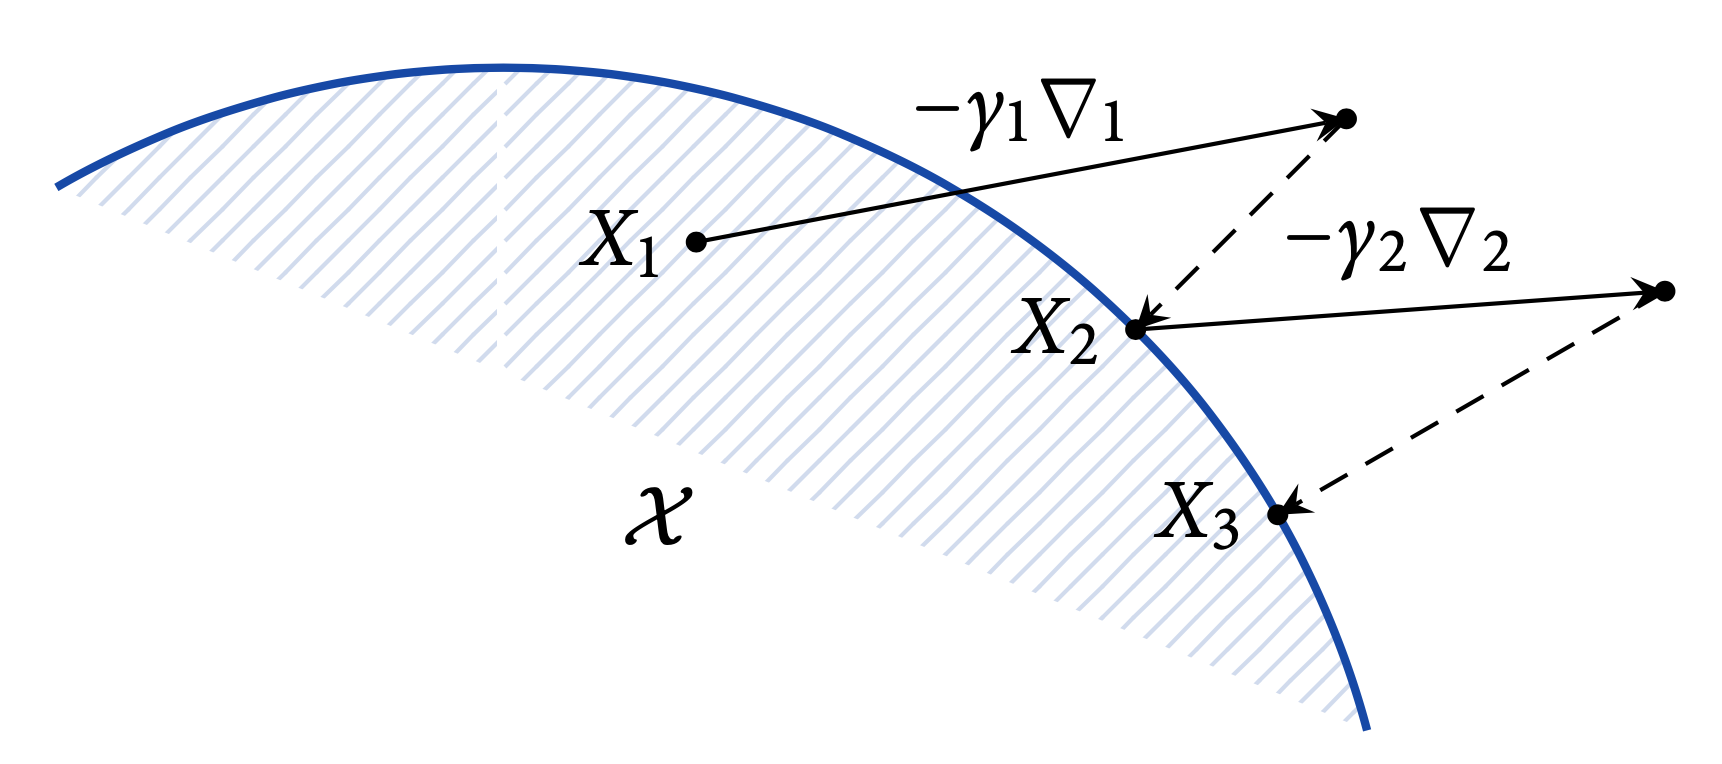
\includegraphics[width=\textwidth]{logos/POGDscheme.png}
  %\captionof{figure}{schematic representation of \ref{equ:POGD}}
  %\label{fig:POGDscheme}
\end{subfigure}
\caption{pseudo code and schematic representation of \ref{equ:POGD}}
\label{fig:POGDpseudoCodeAndScheme}
\end{figure}

It is worth mentioning that the addition $x_t + \gamma_t v_t$ in the update step is not well-defined in general as we add a primal with a dual vector. Assuming $\mathcal{V}$ to be the Euclidean space however, we have that its dual space $\mathcal{V}^*$ is canonically identified with $\mathcal{V}$. This assumption can only be made when the Euclidean $l_2$ norm is used \cite{HDRmertikopoulos}. Lets move to the \textit{regret} analysis of \ref{equ:POGD} \cite[Theorem 2.2]{HDRmertikopoulos}.

\begin{proposition}\label{prop:regretPOGD}
    Suppose \ref{equ:POGD} is run on a sequence of convex and $L_t$-Lipschitz loss function $l_t$ with a constant step size $\gamma_t \equiv \gamma > 0$ where  \textnormal{diam}($\mathcal{X}$) $\equiv$ \textnormal{max}$\{\|x'-x\|:x,x' \in \mathcal{X}\}$ denotes the diameter of $\mathcal{X}$. In particular, if $L \equiv \textnormal{sup}_t L_t < \infty$ and $\gamma = \frac{\textnormal{diam}(\mathcal{X})}{L\sqrt{T}}$, then the regret is bounded by 
    \[reg(T) \le \textnormal{diam}(\mathcal{X})L\sqrt{T}\]
\end{proposition}

We can conclude that up to a multiplicative constant \ref{equ:POGD} enjoys the same \textit{regret} bound as \ref{equ:FTRL} (proposition \ref{prop:RegretFTRL}). Both algorithms have \textit{regret} in the size of $\mathcal{O}(\sqrt{T})$ and are thereby \textit{no-regret} algorithms. \ref{equ:FTRL} however needs \textit{full information} on the loss function $l_t$ at each time step whereas \ref{equ:POGD} just needs \textit{first-order information} in form of the gradient. This makes \ref{equ:POGD} more lightweight and applicable to a wide range of problems \cite{HDRmertikopoulos}. \\

Before we move on let us address the connection between \textit{follow the regularized leader} and \textit{online gradient descent}. Consider the unconstrained linear optimization problem with $\mathcal{X} = \mathbb{R}^n$, Euclidean regularizer $h = \frac{1}{2}\|x\|^2$ with respect to $l_2$ norm and linear losses of the form $l_t(x) = -\langle v_t,x\rangle$ for some sequence $v_t \in \mathbb{R}^n$. According to \ref{equ:FTRL} this yields

\begin{equation*}
    \begin{split}
        x_{t+1} & = \argmin_{x \in \mathcal{X}} \bigg\{\sum_{i=1}^t l_i(x) + \frac{1}{\gamma}h(x)\bigg\} = \argmin_{x \in \mathbb{R}^n} \bigg\{\|x\|^2 - 2\gamma\sum_{i=1}^t \langle v_i,x\rangle\bigg\} \\
        & = \argmin_{x \in \mathbb{R}^n} \bigg\|x - \gamma\sum_{i=1}^t \langle v_i,x\rangle\bigg\|^2 = \gamma\sum_{i=1}^t v_i = \gamma\sum_{i=1}^{t-1} v_i + \gamma v_t = x_ + \gamma v_t
    \end{split}
\end{equation*}

That is simply the unprojected update policy of \ref{equ:POGD}. Its an example of a much more general link between \textit{leader following} and \textit{gradients} dynamics. The main idea is to "linearize" \ref{equ:FTRL} in a sense that we replace $l_t(x)$ with its \textit{linear surrogate} $\Tilde{l}(x)$.

\begin{equation*}
    \Tilde{l}_t(x) = l_t(x_t) + \langle \nabla l_t(x_t),x_t-x \rangle
\end{equation*}

Applying the linear surrogate to \ref{equ:FTRL} leads to \textit{follow the linearized leader} \ref{equ:FTLL} \cite{HDRmertikopoulos}. 

\begin{equation}
    \tag{FTLL}
    x_{t+1} = \argmax_{x \in \mathcal{X}} \bigg\{\gamma\sum_{i=1}^t v_s - h(x)\bigg\}
    \label{equ:FTLL}
\end{equation}

The signal $v_s$ simply denotes the perfect gradient of the loss function $l_t$ at $x_t$ just like in equation \ref{equ:gradient}. Note that by this modification \ref{equ:FTLL} only requires first order information just like \ref{equ:POGD}. Writing \ref{equ:FTLL} recursively leads to the \textit{dual averaging} framework. For more details on that refer to \cite{HDRmertikopoulos, mertikopoulos}.


\section{Online Mirror Descent}\label{section:OnlineMirrorDescent}

As discussed in \cite{shalev, HDRmertikopoulos} there are cases where the problem's geometry may allow considerably sharper \textit{regret} as in \ref{equ:POGD}. In the \textit{multi-armed bandit} problem, for instance, when using Euclidean norm the Lipschitz constant $L$ can be bounded by $\sqrt{n}$. Using $l_\infty$ norm instead of $l_2$ norm, however, we can bound $L$ by $1$. For a more detailed survey on this refer to \cite{shalev, HDRmertikopoulos}. The natural question arises whether running \ref{equ:POGD} with non-Euclidean norm can lead to better \textit{regret} bounds. That question is addressed by the \textit{online mirror descent} framework. \\

To understand the idea of \textit{online mirror descent} lets revisit \textit{projected online gradient descent} and formulate it in a more abstract way. Given an input point $x \gets x_t$ and an impulsive vector $y \gets \gamma_t v_t$, then \ref{equ:POGD} returns an output point $x^+ \gets x_{t+1}$ defined as

\begin{equation}
\begin{split}
x^+ = \Pi(x + y) & = \argmin_{x' \in \mathcal{X}}\bigg\{\|x + y - x'\|^2\bigg\} \\
 & = \argmin_{x' \in \mathcal{X}}\bigg\{\|x - x'\|^2 + \|y\|^2 + 2\langle y,x-x'\rangle\bigg\} \\
 & = \argmin_{x' \in \mathcal{X}}\bigg\{\langle y,x-x'\rangle + D(x',x)\bigg\}
\end{split}
\label{equ:EuclideanProj}
\end{equation}

where 

\begin{equation*}
    D(x',x) = \frac{1}{2}\|x'-x\|_2^2 = \frac{1}{2}\|x'\|_2^2 - \frac{1}{2}\|x\|_2^2 - \langle x,x'-x\rangle
\end{equation*}

is the Euclidean distance between x and x'. The function $D: \mathcal{X}\times\mathcal{X} \to \mathbb{R}$ is called \textit{Bregman divergence} and can be generalized by 

\begin{equation*}
    D(x',x) = h(x') - h(x) - \langle\nabla h(x), x'-x\rangle
\end{equation*}

The \textit{Bregman divergence} is induced by some regularization function $h: \mathcal{X} \to \mathbb{R}$. The basic idea of \textit{online mirror descent} is to replace the Euclidean distance in \ref{equ:POGD} by some \textit{Bregman divergence} induced by a regularization function that is not necessarily based on the Euclidean norm. By that we can make use of the problem's geometric properties and hope for a better regret bound. The regularization function can be viewed analogue to the one introduced in \ref{equ:FTRL}, so again we assume $h$ to be continuous and $K$-strongly convex \cite{HDRmertikopoulos}. \\

Depending on the \textit{Bregman divergence} $D$ induced by some regularization fucntion $h$ we can define a more general projection $Q:\mathcal{X}\times\mathcal{Y} \to \mathcal{X}$ named \textit{mirror map} as 

\begin{equation*}
    Q_x(y) = \argmin_{x'\in \mathcal{X}}\bigg\{\langle y,x-x'\rangle + D(x',x)\bigg\} \qquad \forall x\in \mathcal{X}, y \in \mathcal{Y}
\end{equation*}

Finally we can formulate the \textit{online mirror descent} (\ref{equ:OMD}) update policy as follows

\begin{equation*}
    \tag{OMD}
    x_{t+1} = Q_{x_t}(\gamma_t v_t)
    \label{equ:OMD}
\end{equation*}

where $\gamma_t > 0$ again is the step size sequence and $v_t = -\nabla l_t(x_t)$ is the first order information of the loss functions $l_t$ in form of the gradient. Note that the mirror map $Q$ is solely induced by the choice of $h$, the regularization function. Considering the regret analysis of \ref{equ:OMD} we have the following result \cite[Theorem 2.4]{HDRmertikopoulos}

\begin{proposition}\label{prop:regretOMD}
    Suppose \ref{equ:OMD} is run on a sequence of $l_1,\dots,l_T$ of convex loss functions. Further assume each $l_t$ is $L_t$-Lipschitz with respect to some norm $\|\cdot\|$ and $L \equiv \textnormal{sup}_t L_t < \infty$. Let $H \equiv \textnormal{max } h-\textnormal{min } h$ be the "depth" of $h$ and assume $h$ to be $K$-strongly convex and set $\gamma = \frac{1}{L}\sqrt{\frac{2HK}{T}}$. Then we have that
    \[reg(T) \le L\sqrt{(2H/K)T})\]
\end{proposition}

In terms of regret bounds, the main difference between \ref{equ:POGD} (proposition \ref{prop:regretOMD} and \ref{equ:OMD} (proposition \ref{prop:regretPOGD}) is the factor $2H/K$ and the norm defining the Lipschitz constant $L$. The factor fully depends on the choice of the regularizer $h$. So adjusting $h$ to the problem may lead improved efficiency. Lets introduce two examples of regularization functions and their corresponding mirror maps. \\

Consider the \textit{Euclidean regularizer}

\begin{equation*}
    h(x) = \frac{1}{2}\|x\|_2^2
\end{equation*}

with respect to the $l_2$ norm. Obviously the induced mirror map is simply the Euclidean projection in form of equation \ref{equ:EuclideanProj}. In this case \ref{equ:OMD} coincides with \ref{equ:POGD}. 

\begin{equation*}
    Q_x(y) = \argmin_{x'\in \mathcal{X}}\bigg\{\langle y,x-x'\rangle + \frac{1}{2}\|x'-x\|^2\bigg\} = \Pi(x + y)
\end{equation*}

Another commonly used regularization function is the \textit{entropic regularizer}. Let $\mathcal{X} = \Delta(\mathcal{A})$ be the standard probability simplex of $\mathbb{R}^n$. The \textit{entropic regularization} function is defined as

\begin{equation*}
    h(x) = \sum_{a\in\mathcal{A}}x_a\textnormal{log}(x_a)
\end{equation*}

A straight forward calculation shows that $h$ is $1$-strongly convex with respect to the $l_1$ norm \cite{HDRmertikopoulos}. The induced mirror map can be written as

\begin{equation*}
    Q_x(y) = \frac{(x_a\textnormal{exp}(y_a))_{a\in\mathcal{A}}}{\sum_{a\in\mathcal{A}}x_a\textnormal{exp}(y_a)}
\end{equation*}

When we apply this mirror map to the \ref{equ:OMD} framework we obtain an algorithm known as \textit{entropic gradient descent} (\ref{equ:EGD}). For a survey and a more detailed explanation on \ref{equ:EGD} refer to \cite{shalev}. For a pseudo code description and a schematic representation\footnote{borrowed from \cite[Chapter 2]{HDRmertikopoulos}} of \ref{equ:EGD} see figure \ref{fig:EGDpseudoCodeAndScheme}.

\begin{equation}
    \tag{EGD}
    x_{a,t+1} = \frac{x_{a,t}\textnormal{exp}(\gamma_t v_{a,t})}{\sum_{a'\in\mathcal{A}}x_{a',t}\textnormal{exp}(\gamma_t v_{a',t})}
    \label{equ:EGD}
\end{equation}


\begin{figure}[H]
\centering
\begin{subfigure}{.55\textwidth}
    \begin{algorithm}[H]
    \DontPrintSemicolon
    \KwInput{$\gamma_t > 0$, $\mathcal{X} = \Delta(\mathcal{A})$}
    \For{$t = 1,2,\dots,$T} {
    incur loss $l_t(x_t)$ \;
    receive feedback $v_t \gets -\nabla l_t(x_t)$ \;
    update $x_{t+1} = \frac{(x_{a,t}\textnormal{exp}(\gamma_t v_{a,t}))_{a\in\mathcal{A}}}{\sum_{a'\in\mathcal{A}}x_{a',t}\textnormal{exp}(\gamma_t v_{a',t})} \quad \forall a \in \mathcal{A}$ \;
    }
    \end{algorithm}
    %\caption{pseudo code for \ref{equ:POGD}}
    %\label{fig:POGDpseudocode}
\end{subfigure}%
\begin{subfigure}{.45\textwidth}
  \centering
  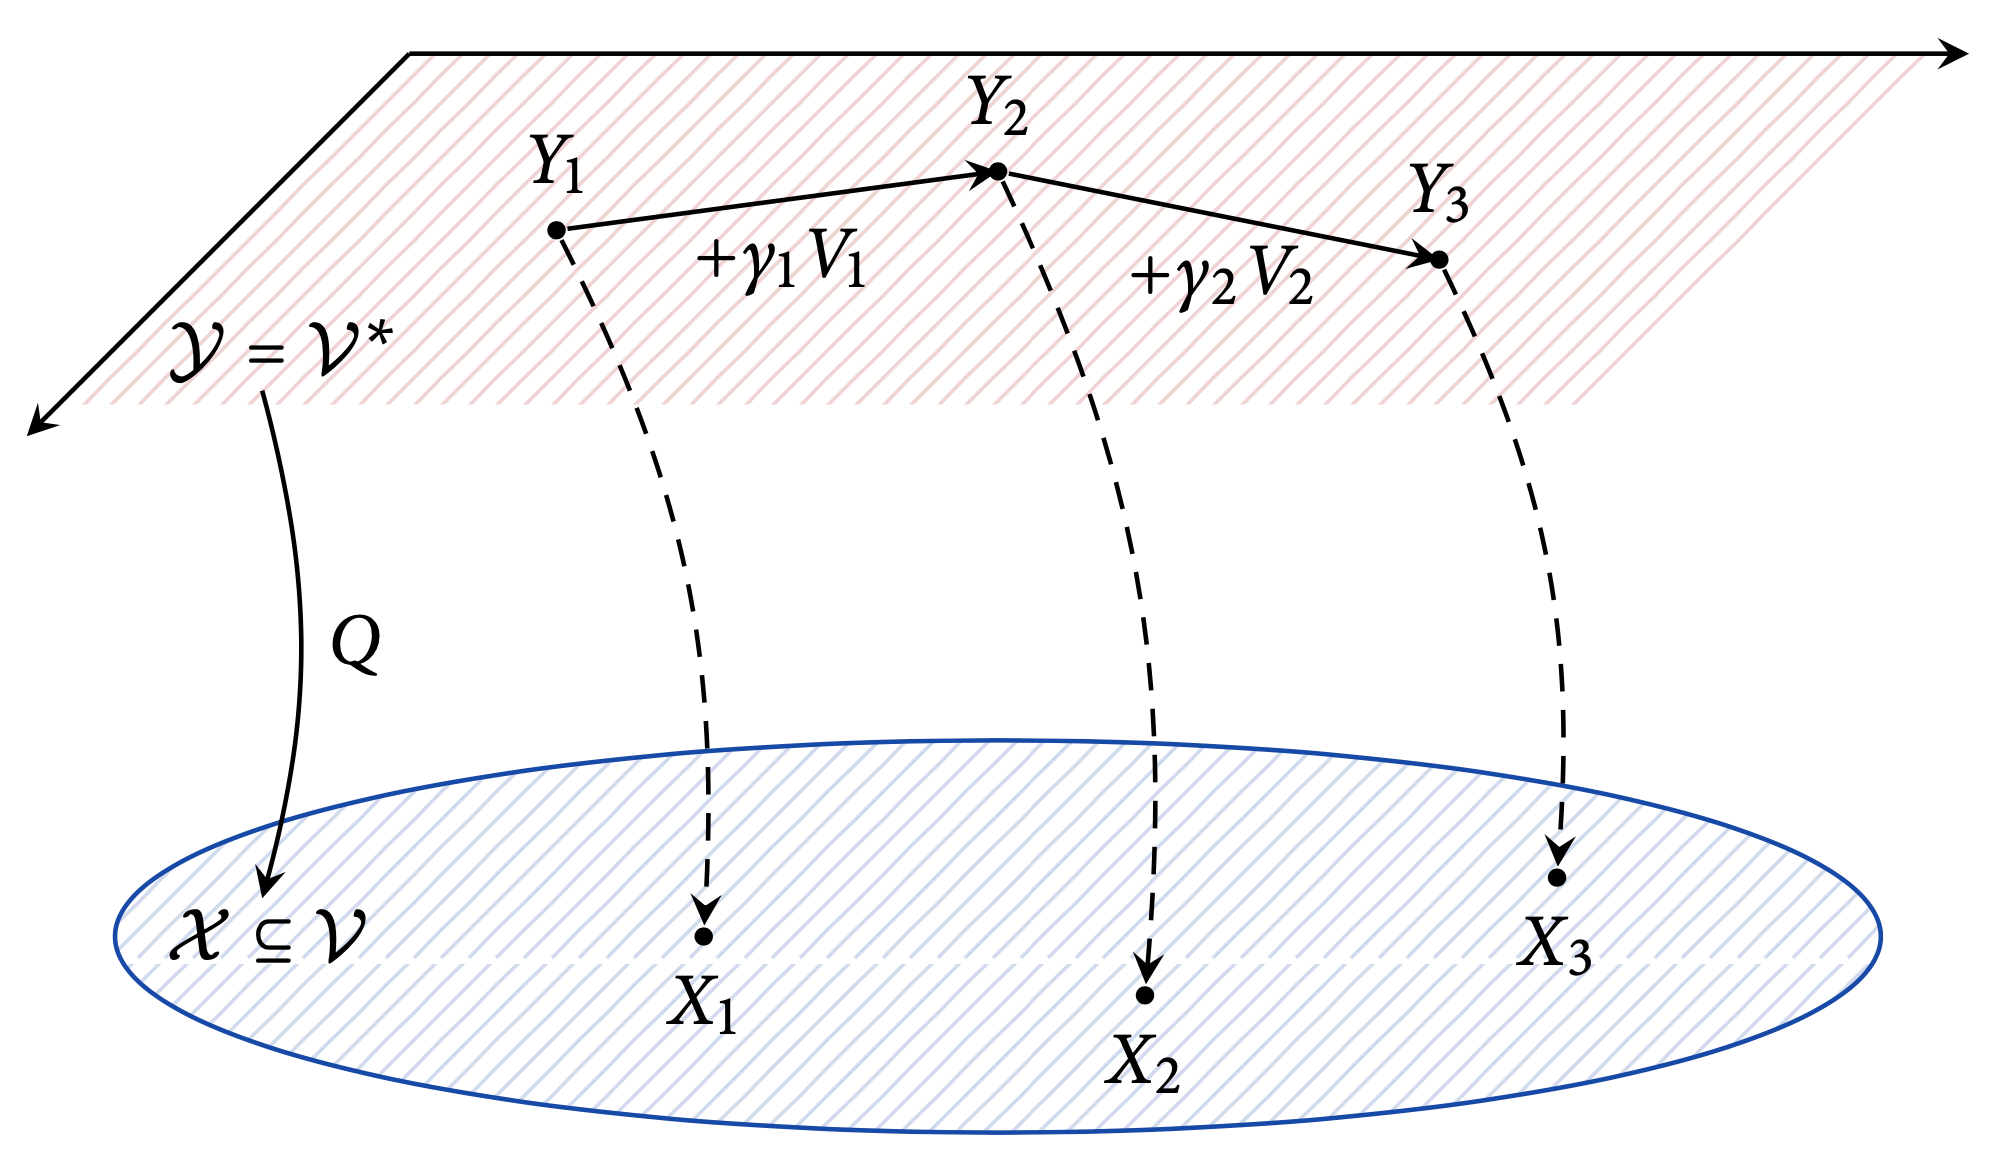
\includegraphics[width=\textwidth]{logos/EGDscheme.png}
  %\captionof{figure}{schematic representation of \ref{equ:POGD}}
  %\label{fig:POGDscheme}
\end{subfigure}
\caption{pseudo code and schematic representation of \ref{equ:EGD}}
\label{fig:EGDpseudoCodeAndScheme}
\end{figure}

An important observation we need to make is that the entropic regularizer becomes infinitely \textit{steep} at the boundary of $\mathcal{X}$. So the effective domain of this regularization function is the relative interior of $\mathcal{X}$, i.e. dom$h$ = ri($\mathcal{X}$). Therefore projections of the mirror map will always return interior points of $\mathcal{X}$ as figure \ref{fig:EGDpseudoCodeAndScheme} suggests. For the Euclidean regularizer, on the other hand, projections lead to points on the boundary of $\mathcal{X}$ like shown in figure \ref{fig:POGDpseudoCodeAndScheme}. The Euclidean regularizer is said to be \textit{non-steep}. \\

Comparing the regret bound between \ref{equ:POGD} and \ref{equ:EGD} in the \textit{multi-armed bandit} problem for example we find that \cite{HDRmertikopoulos}. 

\begin{equation*}
    reg_{POGD}(T) \le 2\sqrt{nT} \qquad \textnormal{and} \qquad reg_{EGD}(T) \le \sqrt{2T\textnormal{log}(n)}
\end{equation*}

As a result, even though both \ref{equ:POGD} and \ref{equ:OMD} enjoy the same regret bound of $\mathcal{O}(\sqrt{T})$ the multiplicative constant involved can have an enormous impact on the speed and efficiency of the algorithm. This can be of of special interest for problems that operate in in high dimensional spaces. \\

By now we have familiarized with the \textit{online mirror descent} framework and encountered two concrete \textit{no-regret} algorithms for constrained problems, namely \textit{projected online gradient descent} \ref{equ:POGD} and \textit{entropic gradient descent} \ref{equ:EGD}. We will later employ these two algorithms on simple two player games and elaborate on their behavior in chapter \ref{chapter:simulations}. Before that let us define finite games formally. 
\begin{comment}

----------------------

\section{The notion of regret}\label{section:theNotionOfRegret}

Convexity is crucial for the design of efficient algorithms. We consider the following online convex optimization framework \cite{shalev}: \\

\begin{figure}[ht]\centering
    \textit{Online Convex Optimization}
    \begin{minipage}{.7\linewidth}
        \begin{algorithm}[H]
        \DontPrintSemicolon
        \KwInput{A $convex$ set $\mathcal{S}$}
        \For{$t = 1,2,\dots,$T} {
        predict strategy $\mathbf{w_t \in \mathcal{S}}$ \;
        receive a $convex$ loss function $f_t:\mathcal{S} \to \mathbb{R}$ \;
        suffer loss $f_t(\mathbf{w_t})$ \;
        }
        \end{algorithm}\caption*{}
  \end{minipage}
\end{figure}


Now, the \textit{regret} of an algorithm measures how "sorry" the learner is, to not have followed a fixed competing strategy in hindsight. It is the difference between the cumulative loss of the sequence of play and the cumulative loss of some fixed strategy. 


\begin{definition}
The \textit{regret} of an algorithm running for $T$ iterations relative to some competing strategy $y \in \mathcal{S}$, is defined as
\[regret_T(y) = \sum_{t=1}^{T}f_t(x_t) - \sum_{t=1}^{T}f_t(y)\]
\end{definition}

Clearly, we want to minimize the \textit{regret} with respect to the best fixed strategy in hindsight. So relative to the set of competing strategies $\mathcal{S}$ the \textit{regret} of an online algorithm is defined as 

\begin{equation*}
    regret_T(\mathcal{S}) = \max_{y \in \mathcal{S}} regret_T(y)
\end{equation*}

The learner's goal is to have the lowest \textit{regret} possible. In fact, we say an algorithm exhibits \textit{no-regret} if the difference between the cumulative loss of the sequence of play and the cumulative loss of the best fixed strategy tends to zero as $T$, the number of iterations, goes to infinity.

\begin{definition}
    An algorithm exhibits \textit{no-regret} iff $regret_T(\mathcal{S})$ grows sublinearly  with $T$, that is
    \[\text{\textit{no-regret}} \Leftrightarrow regret_T(\mathcal{S}) = o(T)\]
\end{definition}


\section{Follow the Regularized Leader}\label{section:followTheRegularizedLeader}

A natural learning rule is to use the one strategy, which had minimal loss on all past rounds. In formulas the update looks like this.

\begin{center}
    \textit{Follow the Leader (FTL)}  
\end{center}
\begin{equation*}
    x_t = \argmin_{x \in \mathcal{S}}\sum_{i=1}^{t-1}f_i(x) \quad \forall t  
\end{equation*} \\

In the first round we can play any feasible strategy and ties can be broken arbitrarily. While this approach yields \textit{no-regret} for some loss functions \cite[Cor. 2.2]{shalev}, FTL does not guarantee \textit{no-regret} in all cases. Consider the following counterexample as in \cite[Ex. 2.2]{shalev}. \\

Let $\mathcal{S} = [-1,1] \subset \mathbb{R}$ and consider the sequence of linear functions such that $f_t(w) = z_tw$ where

\begin{equation*}
    z_t = \begin{cases}
    -0.5 &\text{if $t = 1$}\\
    1 &\text{if $t$ is even}\\
    -1 &\text{if $t > 1 \land t$ is odd}
    \end{cases}
\end{equation*} \\

Apart from $t = 1$, where $z_t$ could actually be set arbitrarily in $[-1,1]$, the predictions of FTL will lead to $w_t = 1$ when $t$ is even and $w_t = -1$ when $t$ is odd. Therefore the cumulative loss of FTL will be $T$, while the cumulative loss of the fixed solution $u = 0 \in \mathcal{S}$ is $0$. Hence, the \textit{regret} of FTL is $T$, which is obviously not sublinearly with $T$. \\

In some sense, FTL seems to be "unstable". The predictions shift drastically from round to round. One way to stablize FTL is to add a so called regularization term. It makes sure that the prediction in the upcoming round is not too "far" off from the current one. 

\begin{definition}\label{def:regularizer}
    A function $R:\mathcal{S} \to \mathbb{R}$ is called regularization function if
    \begin{enumerate}
    \item $R$ is continuous
    \item $R$ is $\sigma-$strongly convex for some $\sigma > 0$
\end{enumerate}
\end{definition}

Using regularization we can define the Follow the Regularized Leader framework as follows

\begin{center}
    \textit{Follow the Regularized Leader (FoReL)}    
\end{center}
\begin{equation}\label{FoReL}
    x_t = \argmin_{x \in \mathcal{S}}\sum_{i=1}^{t-1}f_i(x) + R(x) \quad \forall t
\end{equation} \\

In the upcoming subsections we will introduce two types of regularizations, the Euclidean and the entropic. Euclidean regularization will lead to what is known as Online Gradient Descent, whereas the entropic regularization provides an instance of Online Mirror Descent. Obviously, different regularization terms give different \textit{regret} bounds. We will discuss them later as well. 


\subsection{Online Gradient Descent}\label{subsection:onlineGradientAscent}

Consider the Online Linear Optimization problem where $f_t(x) = \langle x,\boldsymbol{z}_t \rangle$ and let $\mathcal{S} = \mathbb{R}^d$. Applying Euclidean (or $l_2$) regularizer to FoReL will lead to Online Gradient Descent. 

\begin{definition}\label{def:euclideanReg}
    For some step size $\gamma > 0$ the Euclidean (or $l_2$-) regularization term is defined as
    \[R(x) = \frac{1}{2\gamma}\|x\|_2^2\]
\end{definition}
    

Rearranging the equation in \ref{FoReL} with Euclidean regularization yields the Online Gradient Descent algorithm as follows

\begin{figure}[H]\centering
    \textit{Online Gradient Descent (OGD)}
    \begin{minipage}{.7\linewidth}
        \begin{algorithm}[H]
        \DontPrintSemicolon
        \textbf{parameter: }  step size $\gamma > 0$ \;
        \textbf{initialize: } $x_1 = \boldsymbol{0}$ \;
        \For{$t = 1,2,\dots,$T} {
        update $x_{t+1} = x_t - \gamma\nabla f_t(x_t)$ \;
        }
        \end{algorithm}\caption*{}
  \end{minipage}
\end{figure}

Intuitively, the OGD algorithm moves $x_t$ in the direction of the minimum of $f_t$, but not too much because it wants to remember the effect of $f_1,\dots f_{t-1}$. This way, OGD is a \textit{no-regret} algorithm in as sense of definition \ref{def:noRegret} \cite[Cor. 2.7]{shalev}. 

\begin{proposition}\label{prop:EuclideanNoRegret}
    Assume that FoReL is run with Euclidean regularization on a sequence $f_1,\dots,f_T$ of convex functions. Further assume each $f_t$ is $L_t$-Lipschitz with respect to $\|\cdot\|_2$ and let $L$ be such that $\frac{1}{T}\sum_{t=1}^{T}{L_t}^2\le L^2$. Then, for $ \mathcal{S} = \{x: \|x\|_2 \le B\}$ and $\gamma = \frac{B}{L\sqrt{2T}}$ we have that
    \[regret_T(\mathcal{S}) \le BL\sqrt{2T} \in o(T)\]
\end{proposition}

The problem with OGD is that it does not guarantee that the predictions $x_t$ will always be in the probability simplex, the positive vectors whose elements sum to $1$. Therefore we cannot apply OGD in a Finite Game, where strategies are considered as probability vectors as we will see in Chapter \ref{chapter:finiteGames}. We somehow have to \textit{project} the predictions back to the probability simplex in this case. In the next section we will discuss two ways to do so, namely Online Gradient Descent with Lazy Projections and Normalized Exponentiated Gradient. 


\subsection{Online Mirror Descent}\label{subsection:onlineMirrorAscent}

for better transition

\begin{itemize}
    \item Moving beyond these steep cases, our model also allows for penalty functions that are (sub)differentiable over the entire simplex without becoming infinitely steep at the boundary. The basic example here is the squared Euclidean distance, which induces a choice map based on closest point projection. In analogue with the logit case, the orbits of this projected reinforcement learning process are solutions (in an extended sense) of the projection dynamics of Friedman [20], another basic model of evolutionary game dynamics. However, the image of the induced projection-based choice map is the entire simplex (rather than its relative interior), so trajectories of play may now enter and exit the boundary of the simplex in perpetuity (\cite{sandholm}) (Introduction)
    
    \item On Entropic regularizazion: Within this framework, our starting point is the following continuous-time exponential learning process: first, each player maintains a vector of performance scores that represent his actions’ cumulative payoffs; these scores are then converted into mixed strategies using a logit rule which assigns choice probabilities in proportion to the exponential of each action’s score.2 According to a well-known derivation, this logit rule amounts to each player maximizing his expected score minus a penalty term given by the (negative) entropy of the chosen mixed strategy. Moreover, under this learning process, mixed strategies evolve according to the replicator dynamics of Taylor and Jonker [58], a fundamental model from evolutionary game theory \cite{sandholm} (Introduction)
    
    \item idea: Just introduce some penalty functions (entropic and euclidean regularization) and then the induced choice maps (NormalizedEG and Projected Gradient Descent)
\end{itemize}

The idea of Online Mirror Descent is to find a link function that \textit{mirrors} the gradient step back to the feasible set. Lets define a link function $g: \mathbb{R}^d \to \mathcal{S}$ as 

\begin{equation}\label{link}
    g(\boldsymbol{\theta}) = \argmax_{x} \langle x,\boldsymbol{\theta}\rangle - R(x)
\end{equation}

where $R(x)$ is the regularization term. We can rewrite FoReL from \ref{FoReL} based on the recursive update rule \cite{shalev}: 

\begin{center}
    \begin{tabular}{ll}
    \textbf{1.} & $\boldsymbol{\theta}_{t+1} = \boldsymbol{\theta}_t - \nabla f(x_t)$\\
    \textbf{2.} & $x_{t+1} = g(\boldsymbol{\theta}_{t+1})$\\
    \end{tabular} 
\end{center}

This yields the Online Mirror Descent Framework. 

\begin{figure}[H]\centering
    \textit{Online Mirror Descent (OMD)}
    \begin{minipage}{.7\linewidth}
        \begin{algorithm}[H]
        \DontPrintSemicolon
        \textbf{parameter: } a link function $g: \mathbb{R}^d \to \mathcal{S}$ \;
        \textbf{initialize: } $\boldsymbol{\theta}_1 = \boldsymbol{0}$ \;
        \For{$t = 1,2,\dots,$T} {
        predict strategy $x_t = g(\boldsymbol{\theta}_t)$ \;
        update $\boldsymbol{\theta}_{t+1} = \boldsymbol{\theta}_t - \nabla f(x_t)$ \;
        }
        \end{algorithm}\caption*{}
  \end{minipage}
\end{figure}
Setting $\mathcal{S}= \mathbb{R}^d$ and $g(\boldsymbol{\theta}) = \gamma\boldsymbol{\theta}$ we simply obtain Online Gradient Descent. So OMD is a generalization of OGD. \\

As we focus on Finite Games and mixed strategies later, we need the predictions to be probability vectors. Lets constrain $\mathcal{S}$ to be the probability simplex from now on and denote it by $\Delta$. It is defined as 

\begin{equation*}
    \Delta = \{x: \|x\|_1 = 1 \land x \ge \boldsymbol{0}\}
\end{equation*}

In the following we will introduce two common link functions that mirror the predictions back to $\Delta$. 

\subsubsection{Online Gradient Descent with Lazy Projections}\label{subsubsection:OnlineGradientDescentWithLazyProjections}

Analogue to Online Gradient Descent we update the predictions of the algorithm at each time step moving in the negative direction of the gradient of the loss function. But this time we project the predictions back to the probability simplex using Euclidean projection. The link function $g(\boldsymbol{\theta})$ simply returns the closest point in $\Delta$ relative to the gradient step $\gamma\boldsymbol{\theta}$. Formally, 

\begin{equation*}
    g(\boldsymbol{\theta}) = \argmin_{x \in \Delta} \|x - \gamma\boldsymbol{\theta}\|_2
\end{equation*} \\

By applying this link function to the OMD framework we obtain an algorithm known as Online Gradient Descent with Lazy Projections:

\begin{figure}[H]\centering
    \textit{Online Gradient Descent \\ with Lazy Projections (OGDLP)} 
    \begin{minipage}{.7\linewidth}
        \begin{algorithm}[H]
        \DontPrintSemicolon
        \textbf{parameter: } step size $\gamma > 0$ \;
        \textbf{initialize: } $\boldsymbol{\theta}_1 = \boldsymbol{0}$ \;
        \For{$t = 1,2,\dots,$T} {
        predict strategy $x_t = \argmin_{x \in \Delta} \|x - \gamma\boldsymbol{\theta}_t\|_2$ \;
        update $\boldsymbol{\theta}_{t+1} = \boldsymbol{\theta}_t - \nabla f(x_t)$ \;
        }
        \end{algorithm}\caption*{}
  \end{minipage}
\end{figure}

As shown in \cite[Cor. 2.17]{shalev} the Euclidean projection has no impact on the \textit{regret}. Since OGDLP is induced by Euclidean regularization it enjoys the same \textit{regret} bound as in proposition \ref{prop:EuclideanNoRegret} where $B = 1$ as we consider the feasible set to be the probability simplex. Consequently, OGDLP is considered as a \textit{no-regret} algorithm. The next algorithm yields the \textit{no-regret} property while having a much simpler update rule. Instead of Euclidean it uses entropic regularization.


\subsubsection{Normalized Exponentiated Gradient}\label{subsubsection:normalizedExponentiatedGradient}

Another suitable regularizer for simplex constrained optimization problems is the entropic regularization. It is defined as 

\begin{definition}\label{def:entropicReg}
    For some step size $\gamma > 0$ the entropic regularization term is defined as
    \[R(x) = \frac{1}{\gamma} \sum_{i}w[i]log(w[i])\]
\end{definition}

where $log(\cdot)$ is the natural logarithm. Plugging in the entropic regularization in the link function from \ref{link} and rearranging yields the following mirror whose $i$-th component is the function \cite{shalev}

\begin{equation*}
    g_i(\boldsymbol{\theta}) = \frac{e^{\gamma\theta[i]}}{\sum_{j}e^{\gamma\theta[j]}}
\end{equation*} \\

According to the OMD framework we obtain the following simple update rule \cite{shalev}

\begin{equation*}
    x_{t+1}[i] = \frac{w_t[i]e^{-\gamma\nabla f_t[i]}}{\sum_{j}w_t[j]e^{-\gamma\nabla f_t[j]}}
\end{equation*} \\

The derived algorithm is called Normalized Exponentiated Gradient. Note that we cannot initialize $x_1 = \boldsymbol{0}$ as the entropic regularizer is not defined then. We need to choose some interior point of $\Delta$. \\

\begin{figure}[H]\centering
    \textit{Normalized Exponentiated Gradient (NEG)}
    \begin{minipage}{.7\linewidth}
        \begin{algorithm}[H]
        \DontPrintSemicolon
        \textbf{parameter: } step size $\gamma > 0$ \;
        \textbf{initialize: } $\{x: \|x\|_1 = 1 \land x > \boldsymbol{0}\}$ \; 
        \For{$t = 1,2,\dots,$T} { 
        update $x_{t+1}[i] = \scaleto{\frac{w_t[i]e^{-\gamma\nabla f_t[i]}}{\sum_{j}w_t[j]e^{-\gamma\nabla f_t[j]}}}{27pt} \quad \forall i$ \;
        }
        \end{algorithm}\caption*{}
  \end{minipage}
\end{figure}

Just like OGDLP, NEG is a \textit{no-regret} algorithm in the sense of definition \ref{def:noRegret} \cite[Cor. 2.14]{shalev}.

\begin{proposition}\label{prop:EntropicNoRegret}
    Assume that FoReL is run with entropic regularization on a sequence $f_1,\dots,f_T$ of convex functions. Further assume each $f_t$ is $L_t$-Lipschitz with respect to $\|\cdot\|_1$ and let $L$ be such that $\frac{1}{T}\sum_{t=1}^{T}{L_t}^2\le L^2$. Then, for $ \mathcal{S} = \{x: \|x\|_2 \le B\}$ and $\gamma = \frac{B}{L\sqrt{2T}}$ we have that
    \[regret_T(\mathcal{S}) \le BL\sqrt{2log(d)T} \in o(T)\]
\end{proposition}

Note that in comparison with the \textit{regret} bound of OGDLP as in proposition \ref{prop:EuclideanNoRegret} the \textit{regret} bound of NEG also depends on the dimension of the predictions. As we constrained on the probability simplex we can set $B = 1$. \\

To sum up, we introduced two \textit{no-regret} Algorithms that can be applied for simplex constrained convex optimization problems. First, Online Gradient Descent with Lazy Projections (OGDLP) which was based on Euclidean regularization and second, Normalized Exponentiated Gradient (NEG) induced by entropic regularization. We will run both algorithms in simple finite games later in chapter \ref{chapter:simulations}. Before that, lets define finite games and their equilibira concepts. 



\end{comment}

